\chapter{Szoftvercsomag bővítése}
\label{chap:fejezet4}

\section{Megoszthatatlan Feladatok}

Mivel a SourceMeter eszközkészlet több nagyobb szoftvercsomagból áll, melyeknek csomagon belül, és néhány specifikus esetben csomagon kívül is adódnak függőségek a használt szoftverek között, néhány munkafolyamat oszthatatlannak minősült. Ezek a bővítési folyamatnak kezdeténél voltak jelentősek, mivel a SourceMeter által használt sémák nélkül nem lehet az elemzési folyamatot helyesen lefuttatni. A korábbi fejezetben említett sémák tartalmazzák az elemzéshez szükséges ASG felépítését, ennek módosítása létfontosságú volt a munkafolyamat folytatásához.

\begin{figure}[!htbp]
    \caption{Korábban használt JavaScript Sémából egy részlet}\label{fig:apocalypse}
    \centering
    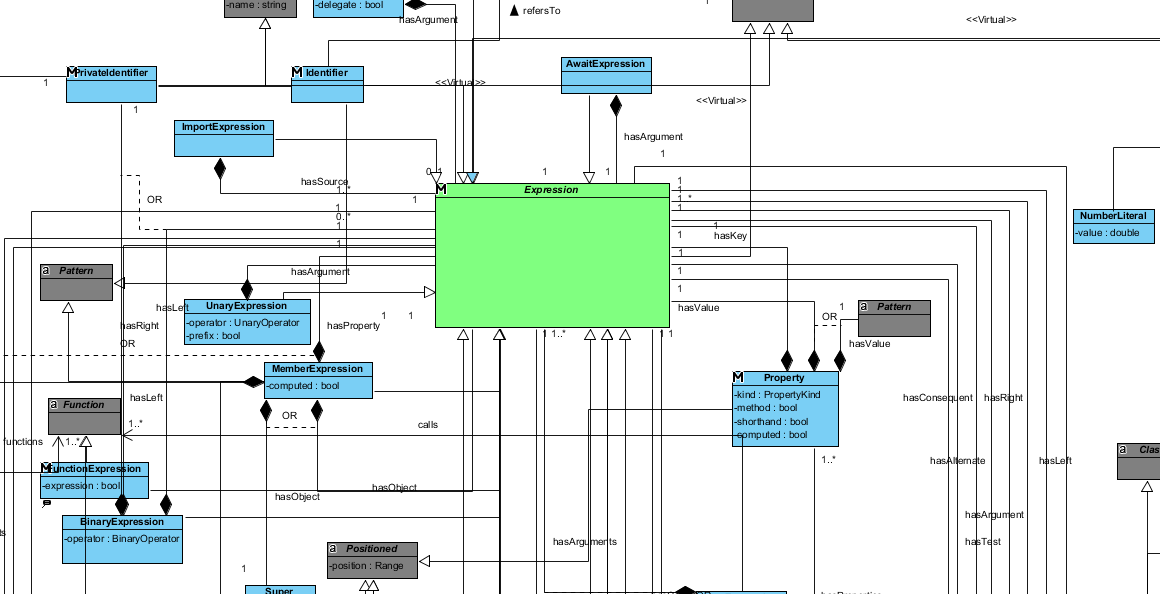
\includegraphics[width=0.9\textwidth]{oldschema.png}
\end{figure}

Az új nyelv támogatásához a typescript-eslint által felvázolt AST \cite{typescript-eslint-ast} alapján hoztunk létre egy új, szervezett formájú sémát. Bár a projektben szerepelt JavaScripthez tartozó séma, a kettő nyelv kompatibilitása ellenére számos eltérés volt jelen az eredeti, ESTree specifikáció \cite{estree-spec} alapján készített és az új, TypeScriptet támogató séma között. Emellett naprakész dokumentáció nem állt rendelkezésre sem a meglévő sémához, sem teljesen új készítéséhez.

Annak érdekében hogy teljeskörű, lehetőleg hibamentes támogatást tudjunk létrehozni az új nyelvnek, egy teljesen új sémát hoztunk létre az új nyelv által használt AST alapján, miközben folyamatosan ellenőriztük a JavaScript kompatibilitást. 

\section{ESLintRunner bővítése TypeScript támogatáshoz}

\subsection{ESLintRunner bevezető}
A SourceMeter for Javascript szoftvercsaládban a forráskód elemzés egyik első lépéseként az ESLintRunner nevű programot futtatja le az elemzendő projekten. Ez a program kimutatja, hogy milyen, előre meghatározott kódolási szabálysértéseket ejtettek a fejlesztés során, és listázza ezen hibák pontos helyét hogy mely fájlokban fordulnak elő, sor és karakter pontosságra. Ezeket egy .xml formátumú fájlba helyezi a program futás után, melyre \aref{lst:eslintoutput}-es ábrában szerepel példa.

\begin{lstlisting}[caption={ESLintRunner kimeneti fájl példa},label={lst:eslintoutput}, language={xml}]
<?xml version='1.0' encoding='utf-8'?>
<ESLintToGraph version='4.3'>
    <file name='C:\\path\\to\\file\\test.ts'>
        <error line='4' column='9' severity='warning' ruleId='no-console' nodeType='MemberExpression' message='Unexpected console statement.' />
        <error line='4' column='9' severity='warning' ruleId='no-undef' nodeType='Identifier' message=' &apos; console &apos;  is not defined.' />
        <error line='4' column='21' severity='warning' ruleId='@typescript-eslint/restrict-plus-operands' nodeType='BinaryExpression' message='Operands of  &apos; + &apos;  operation must either be both strings or both numbers. Consider using a template literal.' />
    </file>
</ESLintToGraph>

\end{lstlisting}

Ez a program egy úgynevezett 'parser', avagy fordító segítségével tudja ezt a feladatát ellátni.

\subsection{Megtett lépések az új nyelv támogatásához}

Ahhoz, hogy TypeScript nyelv elemzésének a támogatását megvalósíthassam, ezen beállításokban megadtam a fordító opciónak ('parser' mező) az újonnan importált 'typescript-eslint' \cite{typescript-eslint} csomagnak a fordító modulját, majd a bővítmények közé ('plugin' mező) a csomag 'eslint-plugin' modulját. 
A bővítmény megadása engedélyezi a programnak, hogy TypeScript nyelvhez kötődő, speciális szabálysértéseket detektálhasson és korábbi, JavaScriptes szabálysértéseket bővítsen ki új, opcionális információkkal. 

Emellett helyes működés eléréséhez szükséges volt megadni az elemezhető fájlok kiterjesztését, melyet a felülbírálásoknál ('overrides' objektum) külön a 'files' és a beágyazott 'parser' mezőkben definiáltam. A mezők egyszerre tartalmazzák a JavaScript (.js és .jsx) és a TypeScript (.ts és .tsx) nyelvekhez tartozó kiterjesztéseket kompatibilitás megőrzése érdekében. Hiányában az alapértelmezett értékek töltődnek be futásidő során a fordítóhoz, mely nem kívánt működésben és eredményekben járulna. Az új fordító esetében azt jelentené, hogy csak TypeScript fájlok elemzése menne végbe.

\begin{lstlisting}[caption={Elemző és bővítmény megadása},label={lst:tsconfig}, language={JavaScript}]
    const typeScriptOptions = {
        ...
        overrides: [
            settings: {
                ...
                import: {
                    parsers: {
                        "@typescript-eslint/parser": ["*.ts", "*.tsx", "*.js", "*.jsx"],
            }}}
        ],
        plugins: [
            "@typescript-eslint/eslint-plugin",
            ...
        ],
        parser: "@typescript-eslint/parser",
    
    \end{lstlisting}

A beállításokhoz szükséges volt új mezők megadása is. A \texttt{parserOptions} mezőn belül szükséges futásidő során a \texttt{project} és a \texttt{tsConfigRootDir} beállítások megadása. A 'project' a TypeScript nyelvben írt projektek konfigurációs fájljainak (névlegesen tsconfig.json) tartalmazza az útvonalait. Ezek alapján tudja az ESLintRunner észlelni, hogy mely fájlokat szükséges elemezni a kódbázisból futásidő során. A 'tsConfigRootDir' mező segítségével megadhatjuk, hogy az előbb beállított konfigurációs fájlok közül melyik tartozik az elemzett projekt gyökérkönyvtárába, ami szükséges adott speciális kódolási szabálysértések helyes működéséhez.

\begin{lstlisting}[caption={Szabálysértések megadása .json állományban},label={lst:jsonconfig}, language={JavaScript}]
parserOptions: {
    ecmaFeatures: {
        jsx: false
    },
    tsconfigRootDir: path.dirname(globals.getOption("inputList")[0]),
    project: [],
    rules: ""
},
\end{lstlisting}

Ahhoz, hogy ezen beállítások futásidő során helyesen be lehessen állítani, elemzés előtt kell átvizsgálni a programmal az elemzendő projektnek a mappaszerkezetét. Mivel formailag kötelező TypeScript projekteknek a gyökérkönyvtárában, így a 'tsConfigRootDir' mező beállítása megegyezik az elemzett projekt útvonalával. Konfigurációs fájlokból viszont egyszerre több is megadható, emiatt a mappaszerkezetben található összes ilyen fájlt meg kell adnunk a 'project' mezőbe. 
A fordító ahhoz, hogy a felhasználók számára megfelelő elemzést biztosítson, csak azokat a fájlokat elemzi alapesetben, melyek a projekt konfigurációs fájljainak az 'include' mezőiben meg vannak adva. Emellett több kisebb hiba javítása is szükséges volt:

\begin{itemize}
    \item Adott fájlok szűrését meg lehet határozni az 'exclude' mezőkben. Továbbá figyelni kellett arra, hogy a konfigurációs fájlokat bővített formátumként kellett kezelni, azaz JSON5-ként. Ez konfiguráció olvasás folyamán megjelenő szintaktikai hibák javítása miatt volt szükséges.
    \item Mivel Linux és Windows operációs rendszereken is futtatható a SourceMeter, ezért adott útvonalakban az elválasztó jeleket általánosítani kellett. Linux rendszereken az útvonalakban a '\textbackslash' jelek karakterfelszabadítást jelentenek, melyek miatt nem létező útvonalakat generálna futás közben a program.
    \item Ritka esetekben akadnak olyan hibák, hogy meglévő konfigurációs fájlok olyan további fájlokra mutatnak, melyek nem léteznek a mappaszerkezetben. Mivel az ilyen esetek hibás elemzési eredményeket generálnak, egy helyettesítő fájlt készítünk. Ez a fájl az elemzés futtatása után törlésre kerül.
\end{itemize} 

\begin{figure}[!htbp]
    \caption{Projekt konfiguráció beolvasás}\label{fig:projconfig}
    \centering
    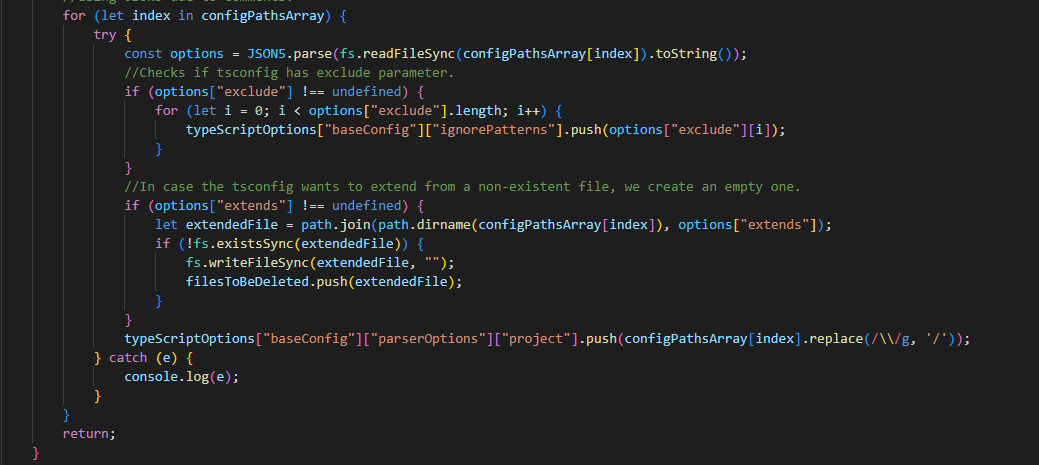
\includegraphics[width=0.9\textwidth]{configreading.png}
\end{figure}

\noindent

Eddigi megvalósítás TypeScript nyelvű projektek elemzésére alkalmas, viszont JavaScript projektek és önálló fájlok elemzésére jelen helyzetben nem alkalmas. Ez abból adódik, hogy ezekben az esetekben nem tartozik az elemzendő kódbázishoz vagy fájlhoz konfigurációs fájl. A probléma megoldására ideiglenes fájlt generál a program (ez nem összetévesztendő a korábban említett ideiglenes konfigurációval, mely egy másik hiba javítására szolgál). Ez a fájl, melynek 'include' mezője tartalmazza projekt esetén a gyökérkonyvtártól számítva a mappaszerkezet összes, kiterjesztésnek megfelelő fájlt, melyek megegyeznek az eddig megadott kiterjesztésekkel a fordító beállításaival. Önálló fájl esetén az 'include' mező csak az elemzett fájlt tartalmazza.
Ilyen elemzések során az ideiglenes konfigurációs fájl van egyedül megadva a 'tsConfigRootDir' mezőben. A fájl az elemzés lefutása után törlésre kerül.
Ezzel a módszerrel a fordító alkalmas egyszerre TypeScript és JavaScript nyelven írt fájlok és projektek elemzésére. 

\begin{figure}[!htbp]
    \caption{Projekt ideiglenes konfiguráció készítése}\label{fig:projtempconfig}
    \centering
    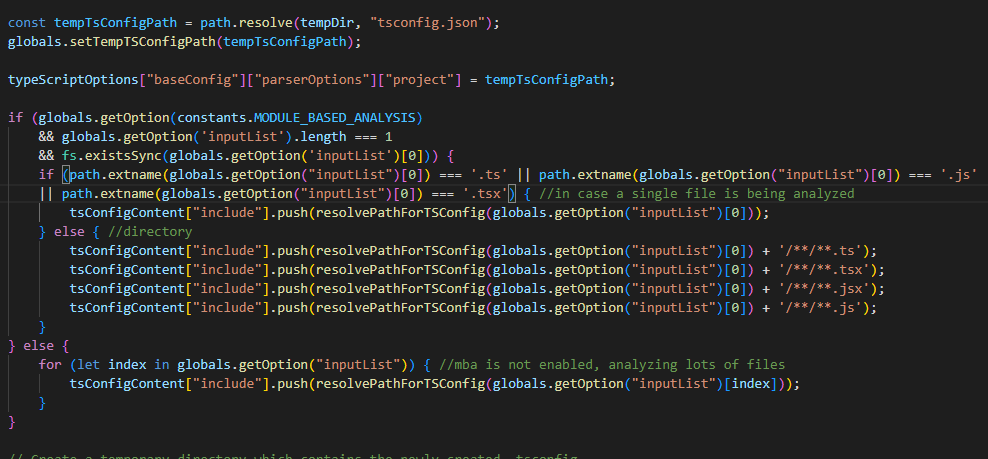
\includegraphics[width=0.9\textwidth]{tempconfig.png}
\end{figure}

Az ESLintRunner futtatásához szükséges használat előtt a programot és a hozzá tartozó modulokat egy önálló fájlba 'összetömöríteni' a webpack nevű szoftvercsomaggal. A program működése TypeScript nyelv támogatás implementálása előtt nem függött külső bővítményektől. Összetömörítés után futás közben az alapértelmezett, 'esprima' nevű fordítóval elemzett, mely az eddig használt modulokba beépítve volt. Az újonnan használt bővítmények használata miatt a program fordítója kényszerítve van külső útvonalak vizsgálatára. A program önmagára nem tud hivatkozni, mivel ezzel az alapértelmezett fordítót használná eddigi implementáció miatt, a modulokat tartalmazó mappát (node\_modules nevű mappa) tömörítés során pedig nem másoljuk át a kimeneti útvonalra. Erre a probléma megoldására többek között a webpack beállításainak módosításával és alternatív kötegelő programok alkalmazásával próbálkoztam. A webpack alternatívák, melyek közé tartozik a Parcel, a Browserify és a Rollup.js, eggyike sem volt alkalmas megoldás, mivel mindegyik hasonló, már webpack használata közben észlelt hibákat állított elő. Észrevehető, egyéb különbségként a használatuk változó nehézsége és gyengébb teljesítményüknek köszönhetően a webpack beállítások módosítása maradt.

Webpack konfigurációban a modul importálások rezolválására használt 'álnevek' (alias) beállítása szolgálhatott volna megoldásul \cite{webpack-resolve}. Ezzel meg lehet adott moduloknak határozni, hogy milyen néven lehessen a programon belül importálni. Ismételt módon a fordító egyedi működésének köszönhetően ez nem használható megoldás, mert a felhasznált pluginokat csak név szerint adjuk meg konfigurációval, nem pedig import utasításokkal.

A végső megoldása ennek a hibának bár egyszerű, később változtatást igényel, amint a fordító program bővítmény kezelésén frissítenek. A program kötegelése során a generált fájl mellé a modulokat tartalmazó mappát is átmásolásra kerül. Ezt a szoftvercsomag fordítása során van elvégezve CMake parancs segítségével. Ennek köszönhetően futásidő folyamán a keresett modult megtalálja és hibamentesen tudja feladatát végezni. Ennek legfőbb hátránya, hogy a program által foglalt hely többszörösére nőtt. A kötegelési módszer változtatása eddigi tesztelések alapján futásidőn nem rontott.

\begin{lstlisting}[caption={CMake parancs modul mappa másolására},label={lst:cmakeeslint}, language={JavaScript}]
    add_custom_command (
        OUTPUT ${EXECUTABLE_OUTPUT_PATH}/node_modules/${PROGRAM_NAME}
        COMMAND ${CALL} npm install > ${CMAKE_CURRENT_BINARY_DIR}/${PROGRAM_NAME}-npm-install.log 2>&1
        COMMAND ${CALL} npm run build -- --no-color -o ${EXECUTABLE_OUTPUT_PATH}/node_modules/${PROGRAM_NAME} > ${CMAKE_CURRENT_BINARY_DIR}/${PROGRAM_NAME}-npm-build.log 2>&1
        COMMAND ${CMAKE_COMMAND} -E copy_directory ${EXECUTABLE_OUTPUT_PATH}/tmp_${PROGRAM_NAME}/node_modules/ ${EXECUTABLE_OUTPUT_PATH}/node_modules/${PROGRAM_NAME}/node_modules/
        ...
    )
\end{lstlisting}

Végül a TypeScript támogatás megvalósításához szükséges volt az új fordító által használt szabálysértések bevezetése a programba. Ehhez kettő különálló fájlt kellett megvalósítanom. A korábban említett .json kiterjesztésű szabály fájl és a \texttt{.rul.md} fájl között legfőbbképp formai eltérések vannak és különböző módon kell őket elkészíteni.

Az alapértelmezett szabály fájl (\texttt{.json} fájl) egy JavaScript objektumot tartalmazó fájl, melyben fel van sorolva a fordítóhoz tartozó összes szabály egy, vagy több hozzárendelt értékkel. A szabályokhoz minden esetben tartozik szám, mely meghatározza, hogy elemzés közben adott szabálysértést detektálni akarjuk-e, és milyen súlyosságot kívánunk hozzá rendelni az elemzés eredményében. Ez az szám 0, 1 vagy 2 értéket vehet fel, 0 esetén átlépi, 1 esetén figyelmeztetésként (warningként), 2 esetén pedig hibaként észleli a program. A második érték, mely nem minden szabálynál található meg, bővebb információt tartalmaz arról hogy pontosan milyen fajtáját detektálja a program. 

\begin{lstlisting}[caption={Szabálysértések megadása .json állományban},label={lst:jsonconfig}, language={JavaScript}]
{ 
  "for-direction": 0,
  "getter-return": [ 0, { "allowImplicit": true } ],
  "no-await-in-loop": 0,
  "no-compare-neg-zero": 1,
  "no-cond-assign": [ 1, "except-parens" ],
  "no-console": [ 1, { "allow": [ "warn", "error" ] } ],
  "no-constant-condition": [ 1, { "checkLoops": true } ],
  "no-control-regex": 1,
  "no-debugger": 1,
  ...
}
\end{lstlisting}

A másik szabály fájl (.rul.md) ugyan ezeket a szabályokat tartalmazza egy átláthatóbb formátumban. Ebben a fájlban a szabálysértésekhez a súlyosságukon kívül kulcsszavak és leírás is tartozik, melyek alapján a szoftvercsomag felhasználói személyre szabhatják az elemzést.
Ennek a szabályfájlnak módosításához korábbi eszközkészlet verziókban egy több lépésből álló folyamat volt. Eredetileg \texttt{.rul} típusú állományokat használtak fel a szabálysértéseket vizsgáló programok. Ezeknek a módosítása során először a módosítandó szabályfájlt '.md' állománnyá kellett konvertálni és a kellő módosításokat Markdown formátumban megírni a fájlban jelen lévő formai követelmények alapján. Ezután a módosított '.md' fájlt html állománnyá (HyperTextMarkupLanguage), majd vissza \texttt{.rul} állománnyá kellett visszaaállítani külső segédprogramok használatával.
Ez a folyamat a jelenlegi eszközkészlet verzión belül jelentősen rövidebb lett. Az új szabályokat a \texttt{.rul.md} állományban formai követelményeknek megfelelően, hosszas konvertálások nélkül lehet implementálni. A szabályokat h2-es fejlécekkel tagolva adjuk meg. Ezen fejléceknél adjuk meg a belső azonosítóját az adott szabálynak, majd alatta h4-es fejlécekkel felsorolva adjuk meg a szabály információit. 

\begin{itemize}
    \item Az 'OriginalId' mező tartalmazza az elemző által felismert szabály nevét.
    \item Az 'Enabled' és a 'Warning' mezők határozzák meg hogy észleljük-e az adott szabálysértéseket, hibaként vagy figyelmeztetésként.
    \item A 'HelpText' mező rövid leírást tartalmaz a szabálysértésről. 
    \item A 'Tags' mező alatt címkéket lehet meghatározni, melyek alapján a szabálysértések kategorizálhatóak.
    \item Az 'OriginalId' mező tartalmazza az elemző által felismert szabály nevét.
    \item A 'Settings' mező alatt néhány szabálysértésnek, mint ahogy korábban az alapértelmezett fájlban meg kellett adni, további információkat is szükséges megadni.
\end{itemize}
 Mivel nyelvre és eszközre szabottak a '.rul.md' fájlok, így csak a '/general/' címkénél szükséges szabályhoz illő értéket megadni, a '/language/' és a '/tool/' címkék megegyeznek. Emellett jelenleg minden szabálysértés, melyet a SourceMeter for JavaScript észlel, 'Settings' mező alatt 'Major', azaz fontos prioritású.

\begin{figure}[!htbp]
    \caption{Szabálysértés megadása .md.rul fájlban}\label{fig:mdszabaly}
    \centering
    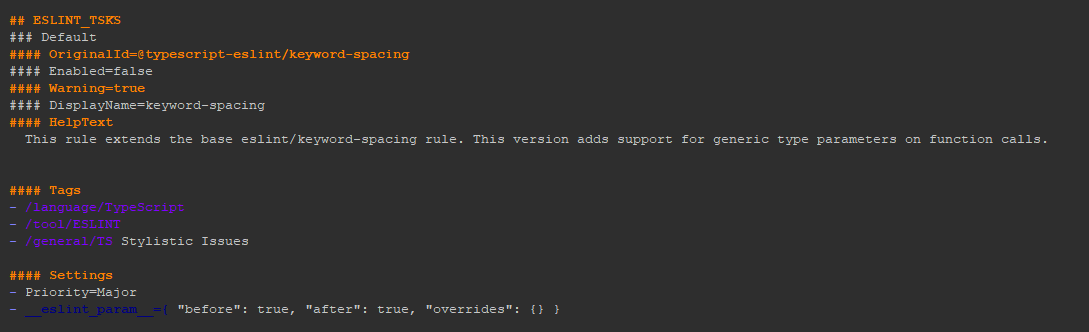
\includegraphics[width=0.9\textwidth]{mdszabaly.png}
\end{figure}

A szabálysértések manuálisan lettek beillesztve, melyek megfelelnek az ESLintRunnerben használt új parser dokumentációjában szereplő információknak. Az, hogy mely szabálysértések vannak engedélyezve elemzés során és szükség esetén ezeknek további részletei megbeszélés alapján voltak meghatározva.

\subsection{Elért eredmények ESLintRunnerben}

\section{JSAN}

\subsection{JSAN bevezető}

Az Analyzer-JavaScript másik alapozó programja a JSAN, avagy a JavaScript Analyzer. Ez a program, mint korábbi fejezetben említve, a bemenetként kapott projekt kódját átalakítja egy egyedi absztrakt szintaxisfává, melyet az elemzés későbbi lépéseiben használunk fel duplikált kódszegmensek keresésére és metrikák kiszámolására.
Ennek a programnak a bővítése jelentősen egyszerűbb ESLintRunnerhez hasonlítva. Az eredeti kódban van egy nagy terjedelmű switch, melyben az elemzés során talált 'csomópontok' (továbbiakban node-ok) típusai vannak felsorolva. Minden felsorolt típushoz tartozik egy külön fájl, mely tartalmazza exportált funkció formájában, hogy a talált node esetén milyen eljárásokat kell elvégezni és milyen adatokat kell beállítani, például egy funkció hívása esetén többek között mi a hozzátartozó név, mik a paraméterei és mi a hozzátartozó kódrészlet. 

\begin{figure}[!htbp]
    \caption{Részlet a JSAN node elemzőjéből}\label{fig:jsanast}
    \centering
    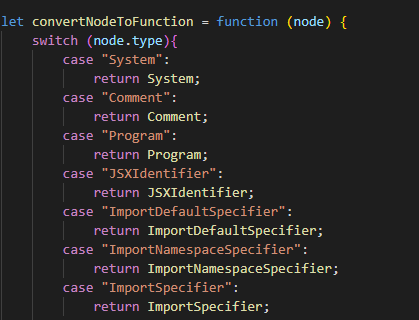
\includegraphics[width=0.6\textwidth]{astswitch.png}
\end{figure}

A program bővítéséhez ezt a switch-et szükséges bővíteni a TypeScript nyelvben található node-ok típusaival, és létre kell hozni ezen típusokhoz tartozó fájlokat.
Ennek a feladatnak a manuális megvalósításával több probléma is fellép. A program karbantarthatósága és olvashatósága jelentősen csökken azzal, hogy több mint 100 új típust vezetünk be az elemzéshez használt switch-be, emellett az említett fájlok manuális megírása vagy módosítása során több hibát is ejthet a fejlesztő, mely miatt a fejlesztési folyamat több időt igényelhet. Manuális fejlesztésre alternatív megoldásként a SourceMeter eszközkészletnek egy segédprogramját, a 'SchemaGenerator'-t olyan funkcióval bővítettem, mely segítségével a szoftvercsomag fordításánál automatikusan legenerálódik a szükséges switch és a hozzá tartozó fájlok. 

\subsection{SchemaGenerator bővítése sablonkód generálással}

A korábban említett segédprogrammal, a SchemaGenerator-ral valósítottam meg az automatikus fájl generálást.
A segédprogram bővítesének célja, hogy sikeresen lehessen generálni több száz node típushoz tartozó fájlt előre meghatározott sablon alapján és a node típusra vizsgáló switchet tartalmazó fájlt, importálásokkal együtt. A fejlesztés folyamatát fokozottan felgyorsította, hogy már korábban használt fájlok generálásához (például szoftvercsomagunk esetén a korábban említett javascriptAddon fájl) már előre meg voltak írva séma bejárására használt funkciók. 
SchemaGenerátoron belül található a 'traversalDescendantBFT()', 'traversalAllEdges()' és a 'traversalAllAttributes()' nevű funkciók. Ezeknek a funkcióknak segítségével lehet bejárni az adott sémákban definiált node típusokat, az ezekhez tartozó attribútumokat és éleket.  


A switch generálása kettő lépésből áll. Először a generált fájlok importálását, majd a típusokat felsoroló switch-et kell legenerálni. Mivel ehhez csak a node-ok nevei szükségesek, a traversalDescendantBFT() funkció kétszeri hívásával ez a feladat egyszerű megoldással rendelkezik.

\begin{lstlisting}[caption={Absztrakt és speciális node szűrés},label={lst:computedfiltering}, style={CStyle}]
bool generateSwitchCase() {
    debugMessage(0, "Generating AST switch...\n");
    file = fopen("ASTSwitchCase.js", "w");
    if (file == NULL) {
        printf("Error opening file!\n");
        return false;
    }
    getFileNamesForImports();
    fprintf(file, "import {default as Literal} from \"./nodes/Literal.js\";\n");
    fprintf(file, "\nlet convertNodeToFunction = function (node) {\n");
    fprintf(file, "    switch (node.type){\n");
    getFileNamesForCases();
    ...
\end{lstlisting}

A kettő bejárás során közel azonos módon dolgozza fel a program az adatokat, mivel csak formailag más az adott node-hoz tartozó kód kiíratása. Bár a két funkció összevonható lenne tartalmuk alapján, kód olvashatóság és későbbi továbbfejleszthetőség miatt külön vannak kezelve.
Ezeken kívül adott dolgokat statikusan kiíratunk a generált fájlba, többek között a switch deklarálását, exportálását, és adott node típusokat a switch-en belül. Sémában definiált, egyedi működés miatt literálokat egy node típusként kezelünk ahelyett, hogy literál fajtánként külön node-okat veszünk fel. Emellett az AST ellenére, melyben a literálok különböző node-okat kaptak, elemzés során minden literál node 'LiteralExpression'-ként van észlelve, és ezt manuálisan szükséges lekezelni.

Node típusok között az AST-n belül találhatóak node párosok, melyek 'Computed' és 'NonComputed' végződésűek. Ezek a node típusok olyan kódolási elemeket foglalnak magukba, melyeknek a hivatkozásaik megadhatóak előre, fordítás előtt statikusan (NonComputed), vagy fordítás során, futásidő közben (Computed) [CITATION HERE].

\begin{lstlisting}[caption={Absztrakt és speciális node szűrés},label={lst:abs-computedfiltering}, style={CStyle}]
if (node->type.abstract && strcmp(node->name, "LiteralExpression") != 0) {
    return true;
}

if (strstr(node->name, "NonComputedName") != NULL) {
    return true;
}
...
\end{lstlisting}

Ezek a node-ok speciális módon vannak megkülönböztetve az AST-ben és a futásidő közben elemzett node-ok között. AST-ben ezek külön-külön bejegyzéseket kapnak azonos tulajdonságokkal, viszont egy ilyen tulajdonságuk név alapján kapnak értéket. A node-ok tartalmaznak egy 'computed' mezőt, mely 'Computed' node-oknál igaz értéket kapnak, 'NonComputed' esetén pedig hamis értéket. Elemzés során viszont ezek a node-ok nincsenek névlegesen megkülönböztetve, de a 'computed' mező alapján különböző típusú node-nak számítanak.
Emellett vannak absztrakt node-ok is meghatározva az AST-ben, melyek a sémában megjelennek mint node-ok, de elemzés során nem jelennek meg. Ezek a fájlgenerálás folyamán kihagyhatóak, kivéve a LiteralExpression, ami absztrakt létének ellenére szükséges, mint összefoglaló node a literál típusokra.

Ezek lekezelése könnyen elvégezhető azzal, hogy névre és adott tulajdonságokra szűrve kihagyunk adott node-ok generálását. 
Ebben az esetben kiszűri az absztakt node-okat, melyeknek a neve nem 'LiteralExpression', majd azokat, melyeknek a neve tartalmazza a 'NonComputedName' szövegrészletet. Azért szűrünk kifejezetten NonComputedName-re, mert a node párosokból legalább az egyikre szükség van hogy helyesen lehessen legenerálni a switchet. Ezekben az esetekben a node nevének végéről a 'ComputedName' szövegrészletet levágódik és úgy illesztődik be a fájlokba.

\begin{lstlisting}[caption={Computed és NonComputed node-ok kezelése},label={lst:abs-compnoncomp}, style={CStyle}]
if (strstr(fileNameWithExtension, "ComputedName")) subStrCopyFunc(fileNameWithExtension, fileNameWithExtension, strlen(fileNameWithExtension) - strlen("ComputedName"));
	strcat(fileNameWithExtension, ".js");
\end{lstlisting}


Az egyes node-okhoz tartozó fájlok legenerálása sokkal több szűréssel és feltétellel jár. Bár legtöbb fájl azonos sablon alapján lesz felépítve, vannak speciális fájlok, mint a Program és a Literal, melyek statikusabb módon épülnek fel. Emellett a 'Computed' és 'NonComputed' node-oknak másképp kell megadni a wrapperjeiket, mivel a két fajta node, bár egyeznek (egy tulajdonság kivételével), mégis külön wrappert kapnak.

Switch generáláshoz hasonlóan itt is le kell szűrni az absztrakt és a NonComputed node-okat, az előző funkciókhoz hasonló módon.
Adott, minden node esetén megjelenő tulajdonság kiíratása után le kell generálnunk a first visit-be tartozó tulajdonságok settereit, és az él metódusok settereit. Ezt két külön funkcióval valósítottam meg, mindkettőnek paraméterként megadva a jelenlegi fájl generálásához felhasznált node. 
Ezekkel a funkciókkal bejárjuk az adott node-oknak a first visit attribútumait, és az edge settereit és, mint eddig nevek alapján tettük, tulajdonság nevekre és típusokra szűrve írattatom ki a megfelelő settereket.
First visit attribútumok esetén, mivel adott node-oknál más típusú attribútumok fordulhatnak elő, vagy szituációtól függően máshogy kell beállítani az attribútumokat, ezeket külön külön kiszűrjük futásidő folyamán.

\begin{lstlisting}[caption={Attribútum szűrésről példa},label={lst:attributefilter}, style={CStyle},basicstyle=\fontsize{9}{11}\selectfont\ttfamily]
if (
  (strcmp(currentNode->name, "TSAbstractMethodDefinitionComputedName") == 0 
  || strcmp(currentNode->name, "TSMethodSignatureComputedName") == 0 
  || strcmp(currentNode->name, "MethodDefinitionComputedName") == 0) 
  && strcmp(lowerName, "kind") == 0) {
  fprintf(f, "if (node.%s != null) %s.set%s(
    conversions.convertMethodDefinitionKind(node.%s));\n", 
    lowerName, currentNode->name, upperName, lowerName);}
else if (strcmp(lowerName,"kind") == 0 
  || strcmp(lowerName, "importKind") == 0 
  || strcmp(lowerName, "exportKind") == 0 
  || strcmp(lowerName, "accessibility") == 0) {
  fprintf(f, "if (node.%s != null) %s.set%s(conversions.convertKinds(node.%s));\n", lowerName, currentNode->name, upperName, lowerName);}
\end{lstlisting}

Él setterek esetén csak két esetre szükséges figyelnünk. Mivel minden él setter esetén más node-okat kapnak a legenerált funkciók, így típusra nem szükséges figyelnünk (mivel ez már schemában le van kezelve), kizárólag a multiplicitást kell ellenőriznünk, azaz egy adott node tulajdonsághoz egy nodeot, vagy egy tömbnek a nodejait rendeljük.

\begin{lstlisting}[caption={Él szetterek fájlba írása},label={lst:edgefilter}, style={CStyle}]
if (edge->mult == 1) {
    ...
} else {
    ...
}
\end{lstlisting}

\subsection{Generált fájlok átmásolása}

Miután ezeket a lépéseket minden szükséges nodera elvégeztük, a program áttérhet a fájlok átmásolására megfelelő célmappába.
A generált fájlok átmásolása a projekt fordítása folyamán történik meg. A fájlokat a korábban említett javascriptAddon mellé generáljuk egy mappában, mely struktúrálisan már elő van készítve másolásra, rendelkezik a megfelelő mappaszerkezettel. Korábbi fordításpl során ha a JSAN-t akartuk lefordítani, a SchemaGenerátor automatikusan meg volt hívva javascriptAddon generálására és megfelelő helyre másolására, így az új fájlokat is ehhez a folyamathoz rendeltem. A programhoz tartozó CMakeList-ben adtam meg utasításként a másolási parancsot. Emellett figyeltem arra, hogy a fájlok generálásához szükséges parancsok azután vannak meghívva, amikor az addon fájl, és ezzel együtt az újonnan létrehozott fájlok generálása végbe ment.
Az alább látható ábrán \texttt{-copy\_directory} CMake parancs használatával volt ez megvalósítva.

\begin{lstlisting}[caption={JSAN Cmake utasítások},label={lst:jsancmake}, language={JavaScript}, basicstyle=\fontsize{9}{11}\selectfont\ttfamily]
add_custom_command (
    OUTPUT ${EXECUTABLE_OUTPUT_PATH}/node_modules/${PROGRAM_NAME}
    COMMAND ${CMAKE_COMMAND} -E copy ${EXECUTABLE_OUTPUT_PATH}/javascriptAddon.node ${EXECUTABLE_OUTPUT_PATH}/tmp_${PROGRAM_NAME}/
    COMMAND ${CMAKE_COMMAND} -E copy_directory ${EXECUTABLE_OUTPUT_PATH}/../lib/javascript/addon/ast ${EXECUTABLE_OUTPUT_PATH}/tmp_${PROGRAM_NAME}/src/ast/
    COMMAND ${CALL} npm install ${MSVS_VERSION} > ${CMAKE_CURRENT_BINARY_DIR}/${PROGRAM_NAME}-npm-install.log 2>&1
    COMMAND ${CALL} npm run build -- --no-color -o ${EXECUTABLE_OUTPUT_PATH}/node_modules/${PROGRAM_NAME} > ${CMAKE_CURRENT_BINARY_DIR}/${PROGRAM_NAME}-npm-build.log 2>&1
    WORKING_DIRECTORY ${EXECUTABLE_OUTPUT_PATH}/tmp_${PROGRAM_NAME}
    DEPENDS javascriptAddon ${EXECUTABLE_OUTPUT_PATH}/tmp_${PROGRAM_NAME}
    COMMENT "Rebuilding ${PROGRAM_NAME}"
)
\end{lstlisting}

Az AST-hez tartozó fájlok automatikus legenerálásának köszönhetően a JSAN karbantartása egyszerűbb lett. Jelentősebb AST változtatások esetén nem lesz szükséges az összes node manuális átnézése és ellenőrzése, hanem csak adott sablonokon kell néhány sorral bővíteni vagy módosítani, mely drasztikusan felgyorsítja a folyamatot. Automatikus generálás esetén olyan problémákat is elkerülhetünk, melyek emberi figyelmetlenségből erjednek, például hibás változó deklarálások, melyek könnyen előfordulhatnak többszáz fájl módosítása esetén. Emellett fejlesztés során pár kisebb hibát is észrevettem az AST-ben, melyek javításra kerültek. 

\section{JSCG bővítése}

\subsection{JSCG bevezetés, hiba felvázolása}
A JSCG, mint korábban említve volt, JSAN által van használva hívásgráf előállítására, melyet a szoftvercsomag későbbi eszközei használnak fel például különböző metrikák számolására. A program futtatása JSAN-on belül történik meg, közvetlen miután az elemzett projekthez tartozó kódbázisnak a fájljai alapján elkészült az AST. Ezeket paraméterként átadja a JSAN a JSCG-nek és meghatározza, hogy milyen stratégiával készítse el a hívásgráfot. Jelenleg 'NONE', 'ONESHOT' és 'DEMAND' stratégiák használata áll rendelkezésre, melyek közül a 'ONESHOT' van felhasználva. A stratégiák közötti különbség az interprocedúrális áramlat követésében különböznek. Nevének megfelelően a 'NONE' stratégia ezt nem követi, míg a ONESHOT csak az azonnal meghívott egyszeri lezárások esetében teszi meg.
JavaScript esetében szükséges volt a hívásgráfok legenerálása a nyelv dinamukissága miatt\cite{feldthaus2013efficient}. Ez TypeScript projekteknél is szükséges, mivel JavaScript nyelv bővítésére szolgál.

\subsection{Bővítés, hibajavítás lépései}

A program már rendelkezett kezdetleges TypeScript támogatással, viszont jelentős mennyiségű node lekezelésére nem volt meghatározva működés. Ezen kívül specifikus TypeScript nyelvtani tényezők észlelése esetén hibába futott a program, mivel eddigi implementáció alapján érvénytelen adatot olvasott be. Ezek a változtatások, JSAN-hoz hasonló módon az új typescript-eslint elemző által használt AST specifikáció alapján lett megvalósítva.

Az előző programok bővítése és folyamatos tesztelések során a JSAN futtatása közben a JSCG által kimutatott hibák alapján voltak meghatározva hogy mely node típusoknál volt szükség változtatásra vagy új működés definiálására. Három fő változtatást kellett megvalósítani:

\begin{itemize}
    \item \texttt{PrivateIdentifier} észlelés \texttt{Identifier} helyén, melyek osztályokban metódus és változó definiálásoknál találhatóak
    \item \texttt{Computed} mezők helyes detektálása osztályokon belül
    \item \texttt{TSEmptyBodyFunctionExpression} helyes bekötése
\end{itemize}

A három közül a \texttt{TSEmptyBodyFunctionExpression} helyes bekötése volt az első amit megvalósítottam. A program több helyen node típusra szűrve végez el adott utasításokat. Ezen szűrések között voltak olyanok, melyek adott funkció típusokra volt érvényes, ezeket kiszerveztem külön funkcióba és hozzáillesztettem az új típust. A funkciótípusok és azok kezelése azonos módon történik AST specifikáció alapján, így ezeknél elegendő volt az új típus ilyen módú beillesztése.

\begin{lstlisting}[caption={Funkció típus szűrő},label={lst:jsonconfig}, language={JavaScript}]
function isFunction(nd) {
    return nd.type === 'FunctionDeclaration' ||
        nd.type === 'FunctionExpression' ||
        nd.type === 'ArrowFunctionExpression'
        nd.type === 'ArrowFunctionExpression' ||
        nd.type === 'TSEmptyBodyFunctionExpression'
}
\end{lstlisting}

\texttt{PrivateIdentifier} esetén hasonló módosításokat hoztam létre, ahol \texttt{Identifier} node típust vizsgált a program, helyettesítettem funkcióval, mely \texttt{PrivateIdentifier} és \texttt{Identifier} típusokra szűrt.

\begin{lstlisting}[caption={Identifier típus szűrő},label={lst:jsonconfig}, language={JavaScript}]
function isIdentifier(ndType) {
    return ndType === 'Identifier' ||
    ndType === 'PrivateIdentifier'
}
\end{lstlisting}

\texttt{Computed} mezők teljes körű támogatásának bevezetése működésükből adódóan nem teljesen volt implementálható.
Ezek a mezők TypeScriptben osztályokban, interfészekben és objektumokban találhatóak, és olyan célt szolgálnak, mellyel futásidő során az említett objektumokhoz dinamikusan nevekkel adhatunk meg metódusokat. Kapcsos zárójeleken belül primitív típusok (szöveg, szám) megadása és ezek között elvégezhető műveletek mellett változókat is megadhatunk, melyeknek értékei lesznek felhasználva a metódus nevének meghatározására.

\begin{lstlisting}[caption={Computed mező példa},label={lst:jsonconfig}, language={JavaScript}]
module.exports = {
    ['foobar3']() {
      return 'fizz';
    },
};
\end{lstlisting}

Ebből adódóan pontos bekötéseket a hívásgráfba nem lehet létrehozni, mivel a projekt futtatása nélkül pontos név megadása ezeknek a mezőknek nem lehetséges.
\texttt{FunctionExpression} típusú nodeok esetén, melyek \texttt{Property} típusú nodeból származnak (azaz a korábban említett objektumok valamelyikének egyik metódusaként van deklarálva), adott esetekre definiáltam ideiglenes működést.

Három gyakori esetre szűrtem le működést. Amikor primitív adattípusokkal, vagy azok között valamilyen művelettel volt megadva érték, akkor az említett node-oknak az értékeit állítottam be mint azonosító. Emellett olyan esetben, amikor változó volt értékként megadva, a változó nevét adtam meg azonosítóként.

\begin{lstlisting}[caption={Azonosító beállítás példa},label={lst:jsonconfig}, language={JavaScript}]
if (parent.key) {
    if(parent.key.left && parent.key.right) {
        nd.id = {
            type: 'Identifier',
            name: parent.key.left.value + parent.key.right.value,
            range: parent.key.range,
            loc: parent.key.loc
        }
}
...
\end{lstlisting}

Változtatások után a a kódon belül érintett dokumentációkat felfrissítettem megfelelő külső hivatkozásokkal és AST referenciákkal. Emellett új teszteseteket is létrehoztam helyes működés ellenőrzésére.